\documentclass[11pt]{exam}
\usepackage{amsfonts,amsthm,amsmath,amssymb,mathrsfs,bbm,dsfont,bm,hyperref}
\usepackage{csquotes}\MakeOuterQuote{"}
\usepackage{hyperref}
\setlength{\paperheight}{12in}
\setlength\parindent{0pt}
\usepackage{xcolor}
\parskip=5pt 
\usepackage{scrextend}
\usepackage{graphicx}
\usepackage{anyfontsize}
\usepackage[shortlabels]{enumitem}


\qformat{\textbf{Problem \thequestion}\quad (\thepoints)\hfill}

\hypersetup{
  colorlinks=true,
  linkcolor=blue!50!red,
  urlcolor=blue!70!black
}


\begin{document}


\begin{center}

     \textbf{Bi/BE/CS 183 2022-2023\\ Instructor: Lior Pachter\\ TAs: Tara Chari, Meichen Fang, Zitong (Jerry) Wang \vskip 0.15in Problem Set 9}

\end{center}


 % \vskip 0.15in


Submit your solutions as a single PDF file via Canvas by {\bf 8am Monday March 13th}. 
\begin{itemize}
  \item If writing up problems by hand, please use a pen and not a pencil, as it is difficult to read scanned submission of pencil work. Typed solutions are preferred.
  \item For problems that require coding, Colab notebooks will be provided. Please copy and save the shared notebook and edit your own copy, which you should then submit by including a clickable link in your submitted homework. Prior to submission make sure that you code runs from beginning to end without any error reports.


\end{itemize}

\begin{questions}
\question[50]

In this question, you will investigate a set of simple, nontrivial models of gene regulation, encompassing the initiation of transcription and production of mRNA molecules. You will derive the steady state dynamics for a model of bursty transcription, which happens to result in a negative binomial distribution of RNA in living cells. `Bursty' transcriptional dynamics in particular are common in bacterial and mammalian systems, outlined in \cite{Cai2006-hk}, where RNA molecules are transcribed in distinct bursts, separated by periods of time (see Fig. 1). The distribution of molecules produced in each burst was additionally shown to be geometric (see Fig. 2). \\

\begin{figure}[!htb]
        \centering
        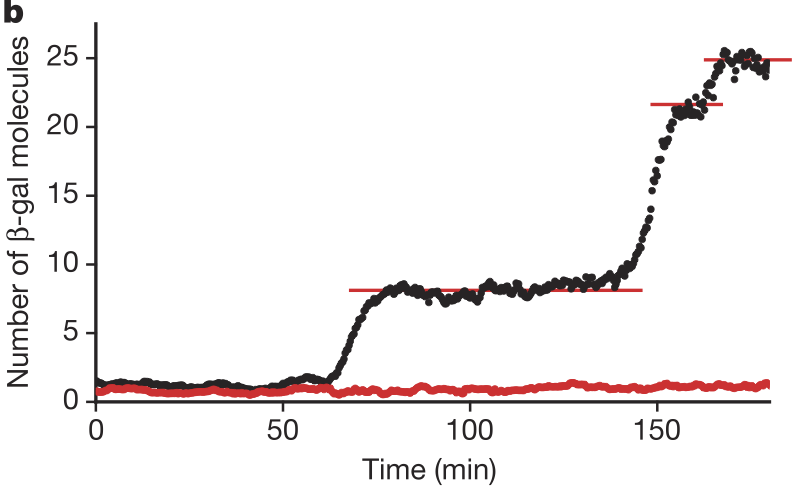
\includegraphics[scale=0.75]{Figures/bursts.png}
        \caption{Number of $\beta$-galactosidase molecules produced, from the $\beta\text{-gal}$ gene in a single cell. Red line denotes a blank background. See also \href{http://be150.caltech.edu/2020/content/lessons/11_bursty.html}{BE150 Bursty Expression} }
    \end{figure}


\begin{figure}[!htb]
        \centering
        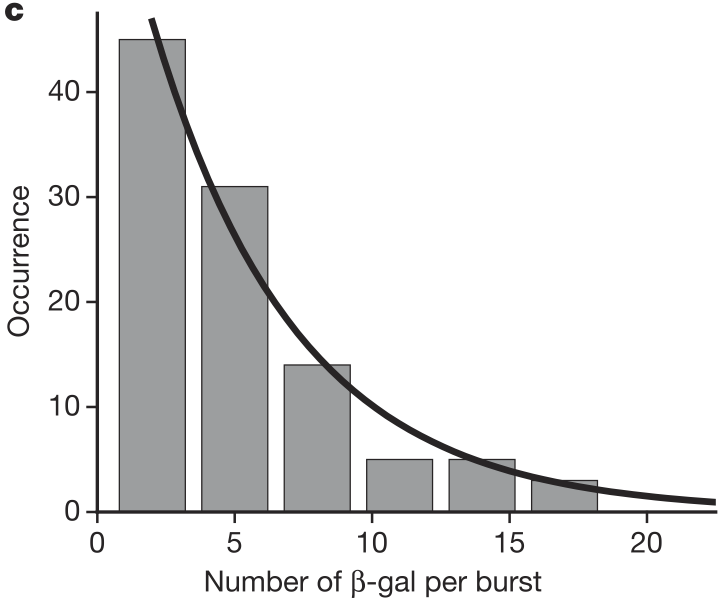
\includegraphics[scale=0.75]{Figures/geom.png}
        \caption{Number of $\beta$-galactosidase molecules produced per burst.}
    \end{figure}



\newpage

To begin the modeling process, we will first define the behavior of a gene that randomly switches between two promoter states: active state $A$ and inactive state $I$. This is known as a telegraph model.
\begin{align}\label{eq:tele}
    \begin{split}
        I &\xrightarrow{k_{on}} A,\\
        A &\xrightarrow{k_{off}} I.
        % A &\xrightarrow{k_{i,A}} A + \mathcal{T}\\
        % I &\xrightarrow{k_{i,I}} I + \mathcal{T}\\
        % \mathcal{T} &\xrightarrow{\gamma} \varnothing
    \end{split}
\end{align}
The promoter transitions from state $I$ to state $A$ with rate $k_{on}$, and from state $A$ back to state $I$ with rate $k_{off}$. We are interested in the probability of the promoter being state $A$ and $I$ at steady state (i.e. when $dP_I/dt = dP_A/dt=0$). Recall from \href{https://docs.google.com/presentation/d/1Nf528xSOGWQS6sEkkAdA1MSt4p7u3aHnttA-tXGlzP0/edit#slide=id.g114859ac4d2_0_156}{Lecture \textbf{17}} that this process is governed by a matrix $\mathcal{A}$, such that $\partial_t P = \mathcal{A}P$, or:
\begin{align}\label{eq:cme_tele}
    \begin{split}
        \frac{d}{dt} \begin{bmatrix}P_I(t) \\ P_A(t)\end{bmatrix} = \begin{bmatrix} -k_{on} & k_{off} \\ k_{on} & -k_{off}\end{bmatrix} \begin{bmatrix}P_I(t) \\ P_A(t)\end{bmatrix}
    \end{split}
\end{align}

\begin{parts}
\part[10] Set the LHS of Equation \ref{eq:cme_tele} to zero and solve for the steady-state probabilities $P_I$ and $P_A$ in terms of $k_{on}$ and  $k_{off}$. Note that $P_I+P_A=1$. 

% We can now introduce some complexity. Each promoter state has an associated transcription rate, $k_{i,I}$ and $k_{i,A}$. This means we can define a \textit{transcription rate process} $K(t)$, which randomly switches between these two values. If $K(t)$ is equal to some constant $K$, we recover the case of constitutive transcription with a constant production rate. 

% It turns out that constitutive transcription is fairly rare. 
\setlength{\parskip}{2em}
% Most genes in bacteria and mammals demonstrate \textit{bursty} RNA transcription: there are intermittent periods of high transcription, separated by long periods of no production at all. This means state $A$ is infrequent, but has a high transcription rate $k_A$. 
Now we will first define the more general stochastic transcription model. We append transcription and degradation reactions to the telegraph system in Equation \ref{eq:tele}:
\begin{align}\label{eq:tele_transc}
    \begin{split}
        I &\xrightarrow{k_{on}} A,\\
        A &\xrightarrow{k_{off}} I\\
        A &\xrightarrow{k_{A}} A + \mathcal{T}\\
        \mathcal{T} &\xrightarrow{\gamma} \varnothing
    \end{split}
\end{align}
where $\mathcal{T}$ denotes a single mRNA molecule. Note we assume transcription only occurs in the active state. \textbf{For a particular duration of the active state $\tau$, the number of mRNA molecules transcribed is distributed according to a Poisson distribution with rate parameter $\tau k_A$.} 

\part[15] Find the distribution for mRNA burst size by integrating over all possible durations of the active state $\tau\in(0,\infty)$. Namely, show that the probability of $x$ transcripts produced while the gene promoter is active is equal to $\alpha_x = (1-p)p^x$ where
$p = \frac{k_A}{k_A + k_{off}}$, meaning that the mRNA burst size takes on a geometric distribution. (Hint: the residence time of every state of a Markov chain is exponentially distributed).  

\setlength{\parskip}{2em}
If now we assume the transcription rates are high but the active state of the promoter is short-lived such that multiple mRNA molecules can be produced instantaneously (taking $k_{off}, k_{A} \to\infty$ while keeping the mean of the mRNA burst distribution finite), we approach the `bursty' limit. We can write down the chemical master equation that governs the number of RNA $n$ as:
\begin{align}\label{eq:cme_burst}
    \begin{split}
        \partial_t P(n,t) &= k_{on} \left[\sum_{x=0}^n \alpha_x P(n-x,t)  - P(n,t)\right] + \gamma \left[(n+1) P(n+1,t) - nP(n,t) \right],
    \end{split}
\end{align}
where $\alpha_z$ is the probability of a burst containing $z$ mRNA molecules part. Our goal is to demonstrate that the limiting distribution $P(n)$ is negative binomial. In principle, we can set the LHS of Equation \ref{eq:cme_burst} to zero, plug in the negative binomial distribution for $P(n)$, and show that the equality holds for some parameter values. Unfortunately, the NB distribution has unwieldy combinatorial factors, and this approach rapidly becomes intractable. Instead, we can use the \textit{probability generating function} (PGF):
\begin{align}\label{eq:pgf_def}
    G(z,t):= \sum_{n=0}^\infty P(n,t) z^n,
\end{align}
where $z\in \mathbb{C}$. By performing the summation over all terms of Equation \ref{eq:cme_burst}, we can convert it to a partial differential equation (PDE):
\begin{align}\label{eq:burst_pgf}
    \frac{\partial G}{\partial t} = k_{on} \left[F(z) - 1\right]G + \gamma \left[1-z\right] \frac{\partial G}{\partial z},
\end{align}
where $F(z)$ is the PGF of the mRNA burst size distribution.

\part[10] Write down the PGF of the burst distribution $F(z)$ by plugging the result from (b) into the definition in Equation \ref{eq:pgf_def}, and calculating the sum.

\setlength{\parskip}{1em}
Now, we can use the PGF of the NB distribution:
\begin{align}\label{eq:nb_pgf}
    G(z) = \left(\frac{1}{1-\theta (z-1)} \right)^r
\end{align}

Now we will find \textit{which} values of $\theta$ and $r$ give us the correct solution.

\part[15] Plug in $F(z)$ from (c) and $G(z)$ from Equation \ref{eq:nb_pgf} into Equation \ref{eq:burst_pgf}, and set its LHS to zero. Solve the resulting equation and calculate $\theta$ and $r$ in terms of $k_{on}$, $\gamma$, and $b$ (where $b$ is the mean of the mRNA burst size). 
\end{parts} 

% Congratulations! You have now demonstrated that there are at least two mechanisms that can lead to a negative binomial distribution of RNA in living cells: ``extrinsic'' cellular heterogeneity and ``intrinsic'' bursting transcriptional dynamics. 

% \question[45]

% In this question, we will apply the CME to solve a simple model of protein translation. To analyze it properly, we should write down a multi-species CME that accounts for (potentially bursty) RNA transcription and degradation, as well as protein translation and degradation. This turns out to be intractable even for the simplest, constitutive model:
% \begin{align}\label{eq:const_with_prot}
%     \begin{split}
%         \varnothing &\xrightarrow{k} \mathcal{T}\\
%         \mathcal{T} &\xrightarrow{\gamma} \varnothing\\
%         \mathcal{T} &\xrightarrow{k_t} \mathcal{T} + \mathcal{P}\\
%         \mathcal{P} &\xrightarrow{\gamma_p} \varnothing,
%     \end{split}
% \end{align} 
% Fortunately, we can make approximations. Proteins have a much longer half-life than RNA, so the variation in RNA levels has a relatively small effect on the relevant timescale. As a zeroth-order approximation, we can write down the following \textit{mean-field} approximation:
% \begin{align}
%     \begin{split}
%         \varnothing &\xrightarrow{k_t \langle T \rangle } \mathcal{P}\\
%         \mathcal{P} &\xrightarrow{\gamma_p} \varnothing,
%     \end{split}
% \end{align}
% where $k_t$ is the translation rate per molecule of RNA, $\langle T \rangle$ is the average number of RNA transcripts, and $\gamma_p$ is the protein degradation rate. This is mathematically identical to the constitutive transcription model, with birth rate $k_t \langle T \rangle$ and degradation rate $\gamma_p$. \\

% The distribution of the protein counts thus follows a Poisson distribution with mean $k_t \langle T \rangle / \gamma_p$, $Poisson(k_t \langle T \rangle / \gamma_p)$. This \textit{discrete} distribution is somewhat unwieldy to evaluate when protein copy numbers are very high, often the case in living cells. To simplify evaluation, we use \textit{continuous} distributions that effectively approximate the protein PMF. 

% \begin{parts} 
% \part[4] As the mean $k_t \langle T \rangle / \gamma_p:=\alpha$ increases, what Gaussian distribution does the discrete PMF converge to? \\

% Even if the assumption that RNA is produced and degraded much faster than proteins holds, the approximations are not equally effective. The constitutive Poisson distribution is best for the \textit{microscopic} regime, where protein numbers are low. The distribution in (a) is best for the \textit{macroscopic} regime, where proteins numbers are high. We can fill in the range between these extremes, the \textit{mesoscopic} regime, which works fairly well when protein abundance is moderate. \\

% From the derivation in lecture, we can write down the following stochastic differential equation (SDE) that tracks the number of proteins $N_t$: 
% \begin{align}\label{eq:sde_full}
%     dN_t = (k_t \langle T\rangle -\gamma_p N_t) dt + \begin{bmatrix}
%     \sqrt{k_t\langle T\rangle} \; & -\sqrt{\gamma_p N_t} \end{bmatrix} \begin{bmatrix} dW_t^{(1)} \\ dW_t^{(2)}\end{bmatrix},
% \end{align}
% where $dW_t^{(1)}$ and $dW_t^{(2)}$ are two independent processes that account for the randomly firing reactions. Note that the SDE has a deterministic term, which tracks the mean of the protein number; the random term essentially quantifies fluctuations about this mean. \\

% The SDE in Equation \ref{eq:sde_full} is in the standard drift-diffusion form:
% \begin{align}
%     dN_t = \mu(N_t) dt + \boldsymbol\sigma(N_t) d\mathbf{W}_t,
% \end{align}
% where $\boldsymbol\sigma$ is the \textit{diffusion coefficient}, here the $1\times 2$ matrix in Equation \ref{eq:sde_full}. We would like to find the distribution of proteins in the mesoscopic regime, which is given by the law of $N_t$ as $t\to \infty$. The easiest way to do this is by converting the SDE into a Fokker-Planck equation, which tracks the evolution of \textit{probability densities} $p(x)$ rather than values $N_t$. \\

% The FPE has the following form:
% \begin{align}\label{eq:fpe}
%     \partial_t p(x,t) &= -\partial_x [\mu(x) p(x)] + \partial_x^2 [D(x) p(x)], \text{ such that}\\
%     D(x) &= \frac{1}{2} \boldsymbol\sigma \boldsymbol\sigma^T.
% \end{align}
% In our case, D(x) is a scalar function. 


% \part[9] The variable $x \in (0,\infty)$ represents the amount of protein molecules. Write down $\mu(x)$ and $D(x)$ in terms of their functional dependence on current state $x$, based on Equation 10 and 11. \\
% \part[14] Write $\partial_x \ln p(x)$ as a function of $\alpha$ and $x$. Plug the solution to (b) into Equation \ref{eq:fpe}.  Since we are concerned with the steady state, we can start with $0=-[\mu p] + \partial_x [Dp]$ instead of the full second-order FPE (assuming $\lim_{x \to +\infty} p(x) = 0$). \\

% \part[9] Integrate $\partial_x \ln p(x)$ to obtain $p(x)$ as $C f(x)$, where $C$ is a normalization constant you do not need to compute. \\

% \part[9] We have obtained an unnormalized probability distribution. Instead of doing another integral, we can exploit the fact that $p(x)$ is closely related to the gamma distribution:
% \begin{align}\label{eq:gamma}
%     f_\Gamma(x) \propto (x-c)^{a-1} e^{-(x-c)/b},
% \end{align}
% where $a$ is the \textit{shape} parameter, $b$ is the \textit{scale} parameter, and $c$ is the \textit{location} parameter. 

% Rewrite the $f(x)$ you have obtained in (d) in the same form as Equation \ref{eq:gamma}. Calculate $a$, $b$, and $c$ that yield $f(x)$.  \\
% \end{parts} 

% Congratulations! You have developed a non-Gaussian mesoscopic approximation to the constitutive transcription process, and written it in a form that can be calculated by any numerical package with gamma distributions.

\newpage
\question[50]
In this question, we will compare our results to stochastic simulations and see how well the various approximations work. The core of the simulation code is already implemented. It remains for you to write the \textit{propensity functions} that determine the instantaneous rates of the reactions. This amounts to writing down the individual contributions to the efflux rates in the matrix $\mathcal{A}$. For example, consider the constitutive production system with transcription rate $k_A$, degradation rate $\gamma$, and $n$ molecules of RNA i.e. there is no inactive state. At each instant, it will assign a propensity of $k$ to the transcription reaction and $\gamma n$ to the degradation reaction. 

You will also investigate the inverse problem, of fitting parameters given data from a stochastic system. You will use a Markov Chain Monte Carlo approach to approximate parameters for the steady state distribution of a system, given data points sampled from the system.

 \href{https://github.com/pachterlab/BI-BE-CS-183-2023/blob/main/HW9/Problem2.ipynb}{Problem 2 notebook}
 
 %\href{https://github.com/pachterlab/Bi-BE-CS-183-2023/blob/main/HW9/Problem2.ipynb}{The Problem notebook is here}.

 Your edited version of the notebook \textit{must be submitted } for this problem. Reminder to check that your notebook runs all the way through with the the {\tt Runtime} $\xrightarrow{}$ {\tt Restart} and {\tt Runtime} $\xrightarrow{}$ {\tt Run All} commands.



\end{questions}
% \begin{thebibliography}{1}
% \bibitem{Trapnell2015}
% Trapnell, C., 2015. Defining cell types and states with single-cell genomics. {\it Genome research}, 25(10), pp.1491-1498.
% \end{thebibliography}
\end{document}


